\documentclass[../main]{subfiles}
\begin{document}

All these images come from \href{http://www.reddit.com/r/wtfstockphotos}{r/wtfstockphotos}. Thought it might cheer people up a bit rather than just a blank box saying \texttt{figure\_1.jpg}.

For referencing any figures or tables (or equations, or chapters/sections/subsections), use the \verb|\cref| command. Instead of the default Latex referencing, it uses the `cleverref' package, and it is just cleverer than default. Of course, make sure you remembered to put a {\verb|\label{}|} on the thing you are trying to reference, and that you haven't used the same name twice. In \LaTeX\, generally your labels are preceded with \texttt{fig:}, \texttt{eq:}, \texttt{tab:} for figures, equations and tables, and also \texttt{sec:}, \texttt{sub:} for sections and sub-sections. It's not a requirement, it's just good practice!

\section{Figures}

\subsection{Single figure}

When placing a single figure, use location specifiers \verb|[htbp]|. This forces \LaTeX\ to try place the image \textbf{h}ere, at the \textbf{t}op or \textbf{b}ottom of the page, or failing all those, make a new \textbf{p}age.

\begin{figure}[htbp]
\centering

\includegraphics[width=0.66\textwidth]{stock1.jpg}
\caption[A single figure.]{An example of a figure on it's own. Remember kids, don't drink and drive, because if you hit a bump your drink goes everywhere.}
\label{fig:stock1}
\end{figure}

\subsection{Multiple figures/subfigures}

You can also have multiple figures next to each other. The way that they are placed/stacked is basically set by the width of the images. If you have two images each under $0.5$ textwidth, \LaTeX\ will place them next to each other horizontally. If you have three at $0.5$ textwidth, two will go on one row, with the third below, etc. (Generally, you actually want the image width to be slightly smaller than you want, e.g. both $0.45$ for two images, to ensure the captions can wrap correctly.) When placing subfigures, make the overall figure environment use \verb|[htbp]|, but each individual sub image should use \verb|[b]| - this seems to work best.

I've included an example of two rows of two images with \cref{fig:stock2_3_4_5}. Notice with these labels, you can reference the overall figure (\cref{fig:stock2_3_4_5}) or each individual image (\cref{fig:stock3}).   

\begin{figure}
    \centering
    \begin{subfigure}[b]{0.45\textwidth}
        \centering
        
\includegraphics[width=\textwidth]{stock2.jpg}
        \caption{stock image 2}
        \label{fig:stock2}
    \end{subfigure}
    \hfill
    \begin{subfigure}[b]{0.45\textwidth}
        \centering
        
\includegraphics[width=\textwidth]{stock3.jpg}
        \caption{stock image 3}
        \label{fig:stock3}
    \end{subfigure}
    \hfill
    \begin{subfigure}[b]{0.45\textwidth}
        \centering
        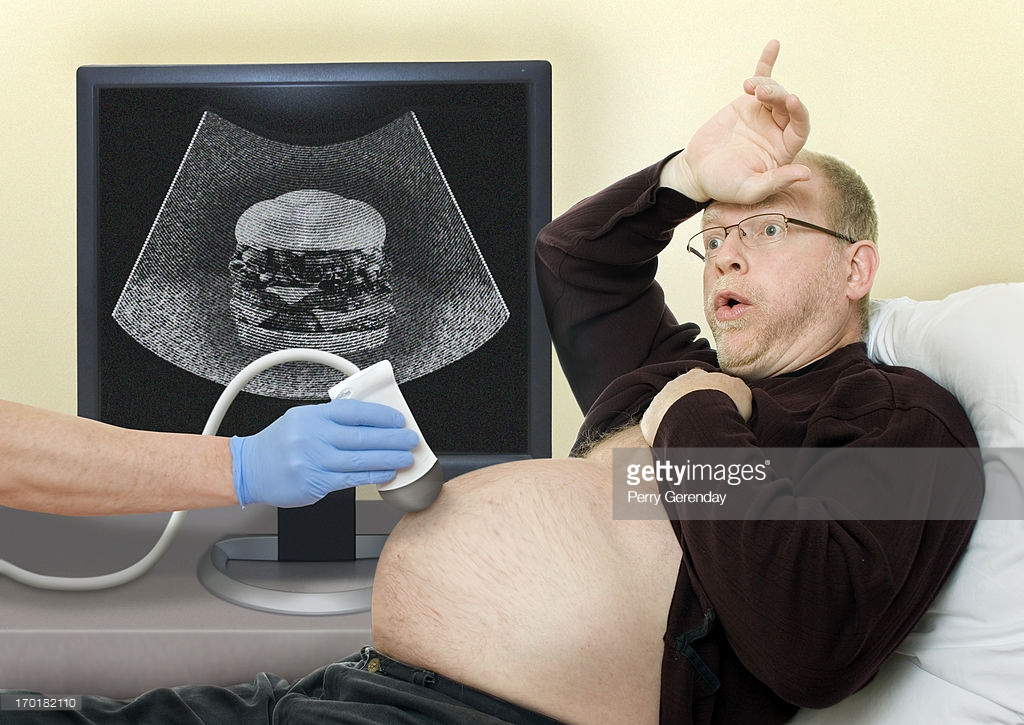
\includegraphics[width=\textwidth]{stock4.jpg}
        \caption{stock image 4}
        \label{fig:stock4}
    \end{subfigure}
    \hfill
    \begin{subfigure}[b]{0.45\textwidth}
        \centering
        
\includegraphics[width=\textwidth]{stock5.jpg}
        \caption{stock image 5}
        \label{fig:stock5}
    \end{subfigure}
    \caption[Sub figures]{And here are some sub-figures done with yet more stock images.}
    \label{fig:stock2_3_4_5}
\end{figure}

\section{Tables}

The key to decent looking tables is that ``less is more''. You should NEVER have a vertical line in a small table\footnote{Unless it has \emph{lots} of text/long sentences, in which case vertical lines might be a good idea - but even then, see \cref{tab:landscape} which doesn't have any.} (if you do, you should probably split into multiple tables). The only horizontal lines you need are the \verb|\toprule|, a few \verb|\midrules| if needed, and a \verb|\bottomrule|. Any more and your tables may become hard to read. Compare the two tables of \cref{tab:ra_dec_lims} and you'll see what I mean.

Inside \texttt{tabular} environments, you seperate columns with \verb|&| symbols. So, if you actually need an \& in your text, do \verb|\&|.\footnote{This goes for aligning equations in maths mode too, see \ref{sec:equations}.}

\subsection{Multiple tables/subtables}\label{sub:subtables}

These two tables, \cref{tab:ra_dec_lims}, are included in a subfile, so that it doesn't take up a bazillion lines in the main editor. Again, like the subfigures, you can reference each individual subtable \cref{tab:uclo_lims} and \cref{tab:km60_lims}. These tables also show off `multicol', in that you can have cells merged along multiple columns. (You can do the same thing with rows.)

% Our table is in a subfile
\subfile{tex/tab_subfile.tex}


\subsection{Decimal alignment in tables}

\Cref{tab:decimals} is aligned around the decimal points of the numbers.

\begin{table}[htbp]
\centering
    \begin{tabular}{r@{.}l}
    \toprule
    \multicolumn{2}{c}{Value} \\
    \midrule
    3   & 14159 \\
    16  & 2     \\
    123 & 456   \\
    \bottomrule
    \end{tabular}
\caption{Aligned round a decimal point.}
\label{tab:decimals}
\end{table}

\subsection{Multicol/multirow/merged cells}\label{sub:merged_cells}

\Cref{tab:multirow} shows off multi-row tables. We've actually already seen multicolumn tables used in \cref{tab:ra_dec_lims} in \cref{sub:subtables}. This functions visually much like ``merged-and-centred'' cells in Excel spreadsheets.

\begin{table}[htbp]
\centering
    \begin{tabular}{lll}
    \toprule
    \multicolumn{3}{c}{Team sheet} \\
    \midrule
    Goalkeeper & GK & Paul Robinson \\ \midrule
    \multirow{4}{*}{Defenders} & LB & Lucas Radebe \\
     & DC & Michael Duburry \\
     & DC & Dominic Matteo \\
     & RB & Didier Domi \\ \midrule
    \multirow{3}{*}{Midfielders} & MC & David Batty \\
     & MC & Eirik Bakke \\
     & MC & Jody Morris \\ \midrule
    Forward & FW & Jamie McMaster \\ \midrule
    \multirow{2}{*}{Strikers} & ST & Alan Smith \\
     & ST & Mark Viduka \\
    \bottomrule
    \end{tabular}
\caption{A table showing off multirow capabilities. Fancy!}
\label{tab:multirow}
\end{table}

\newpage
\begin{landscape}
\subsection{Landscape page for a large table}
I set this page to landscape, because the table is way too wide for a single page otherwise. See \texttt{large\_table.tex} for the code. Also, notice how great this table looks with no vertical lines eh? \emph{You never need vertical lines!}
\subfile{tex/tab_large.tex}
\end{landscape}

\pagestyle{fancy}

\end{document}
